\documentclass[11pt,a4paper,draft]{article}
\usepackage{geometry}
\geometry{letterpaper, portrait, left=1in, right=1in, top=1in, bottom=1in}
\usepackage[latin1]{inputenc}
\usepackage{amsmath}
\usepackage{amsfonts}
\usepackage{amssymb}
\usepackage{multicol}
\usepackage{enumitem}
\usepackage{lipsum}
\usepackage[final]{graphicx}
\DeclareGraphicsExtensions{.pdf,.png,.jpg}
\usepackage[english]{babel}
\usepackage{csquotes}
\usepackage{hyperref}
\usepackage[backend=bibtex]{biblatex}
\bibliography{mybib}
\begin{document}
	\title{Design Review - Team N64}
	\author{Neil Ryan, Steven Kool, Rachel Yanovsky}
	\maketitle
	\newpage
	
	\section{Overview}
	The GameBoy Advance (GBA) was an extremely popular handheld console by Nintendo, released in 2001, succeeding the GameBoy Color. As with previous Nintendo handheld consoles, it was a single-player device, with the option of attaching a link cable between devices for multiplayer interactions. The serial port on the top of the device that the link cable attached to was also used for a wireless adapter in \textit{Pokemon: Fire Red and Leaf Green}, as well as for links between the Nintendo GameCube and the GameBoy Advance. The GameBoy Advance was also backwards compatible with GameBoy Color games.\\\\
	
	The Game Boy Advance (GBA) is composed of four major subsystems - the ARM7TDMI CPU, the graphics pipeline, the sound engine, and the Link Cable serial interface. The GBA also includes a Zilog Z80 processor for backwards GameBoy Color compatibility. Additionally, the Game Boy Advance contains a Direct Memory Access (DMA) controller, several programmable timers, an interrupt controller, and 10 buttons. The graphics pipeline outputs to a 240x160 RGB LCD screen; the sound outputs to either a mono speaker, or the GBA's stereo headphone jack. The system clock is the same as the CPU clock, running at 16.78MHz.\cite{GBAManual} \\\\	
	On a high level, the GBA architecture is a MMIO register based system. The ARM7TDMI acts as a master to configure the various subsystems. Generally, registers act as control points, but are occasionally used to give the status of subsystems to the CPU.\\\\
	Initially, we had planned to finish the semester with a working GameBoy Advance that could play three games: Pokemon Ruby, Legend of Zelda: Minish Cap, and Kim Possible 3: Team Possible (the favorite childhood games of our group members), but several aspects of the project ended up taking much, much longer than we anticipated. We feel, however, that enough dense roadblocks have been dealt with to make this a very achievable project for future groups to complete.\\\\
	
	
	\subsection{Architecture}
	While the GBA generally operates in a master-slave fashion, there are several points of interactions between the subsystems. For the most part in this project, we made no attempt to create a cycle accurate system. It is possible that some games exist that abuse the specifics of the hardware enough to make this a problem, but from our understanding of the GBA specification, there is little incentive to cut game timing close enough to make this a problem - the "hacky" characteristics of some 80s arcade cabinets are unlikely to be present in the GameBoy Advance. Namely, games are likely compiled, instead of hand-assembled.\\\\
	As previously stated, the ARM7TDMI core controls most of the system. 
	
	
	\subsection{GBA Schematic}
	\includegraphics[width=12cm, height=20cm, keepaspectratio=true]{gba_schematic}
	
	\subsection{System Diagram}
	\includegraphics[width=12cm, height=20cm, angle=270, keepaspectratio=true]{system}
	
	\section{Infrastructure}
	\subsubsection{DevKitARM}
	\subsubsection{Emulators}
	\subsubsection{Synthesis \& Verification}

	
	For the most part, we used the standard toolchain - Vivado for synthesis (and occasionally simulation), and VCS for pre-synthesis verification. We also used the \href{http://devkitpro.org/wiki/Getting_Started/devkitARM}{DevKitARM} toolchain for compiling programs to run on the GBA's CPU. 
	
	
	
	\section{Memory}
	The Game Boy Advance memory is divided into 11 regions:\\
	\textbf{System ROM}: Mapped from \texttt{0x00000000} to \texttt{0x00003FFF}. Holds the GBA BIOS.\\
	\textbf{CPU External RAM}: Mapped from \texttt{0x02000000} to \texttt{0x0203FFFF}.\\
	\textbf{CPU Internal RAM}: Mapped from \texttt{0x03000000} to \texttt{0x03007FFF}.\\
	\textbf{I/O Registers}: Mapped from \texttt{0x04000000} to \texttt{0x04000807}. MMIO register mappings.\\
	\textbf{Palette RAM}: Mapped from \texttt{0x05000000} to \texttt{0x050003FF}. Stores the color palette.\\
	\textbf{VRAM}: Mapped from \texttt{0x06000000} to \texttt{0x06017FFF}. Video RAM.\\
	\textbf{OAM}: Mapped from \texttt{0x07000000} to \texttt{0x070003FF}. Object (sprite) attribute memory.\\
	\textbf{Game Pak ROM, WS0}: Mapped from \texttt{0x08000000} to \texttt{0x09FFFFFFF}. Cartridge ROM.\\
	\textbf{Game Pak ROM, WS1}: Mapped from \texttt{0x0A000000} to \texttt{0x0BFFFFFFF}. Cartridge ROM.\\
	\textbf{Game Pak ROM, WS2}: Mapped from \texttt{0x0C000000} to \texttt{0x0DFFFFFFF}. Cartridge ROM.\\
	\textbf{Game Pak RAM}: Mapped from \texttt{0x0E000000} to \texttt{0x0E00FFFF}. Cartridge RAM.\cite{GBAManual}\\
	
	Memory from \texttt{0x04000000} to about \texttt{0x04000807} is mapped to I/O registers (the programmers manual only lists register mappings up to \texttt{0x04000208}, but hobbyist reverse engineering shows some internal registers up to location \texttt{0x04000800}).
	
	
	Additionally, the upper 1M-bit of each ROM region is used as flash memory.
	
	The three regions for Game Pak ROM are identical mappings, the difference is the number of wait states used in the access (see Memory Interface). We plan to use the Zedboard's Block RAM for the System ROM,  CPU Internal RAM, Palette RAM, VRAM, and OAM regions. We plan to use the Zedboard's DDR3 RAM for the Game Pak ROM, the Game Pak RAM, and the CPU External Working RAM. MMIO registers will be implemented with the Zedboard fabric SRAM. At system reset, the SD card controller will write the contents of the SD card to DRAM. Given that the CPU's clock is only at 16.78Mhz, we can drive our DRAM controller with a sufficiently fast clock to make DRAM accesses appear single cycle from the CPU's perspective. The various memories have different bus widths - to accommodate, the bus includes a \texttt{SIZE[1:0]} - where 3 corresponds to a word (32 bits), 2 to a half word (16 bits), and 1 to a byte (4 is reserved). When reading, the lowest two bits of the address will be used to determine the specific memory location, when writing, the combination of the lowest two address bits and \texttt{SIZE[1:0]} will be used to address specific locations.\\
	\subsection{Memory Regions Bus Widths}
\begin{center} %TODO Include picture of bus widths
	\begin{figure}[ht!]
	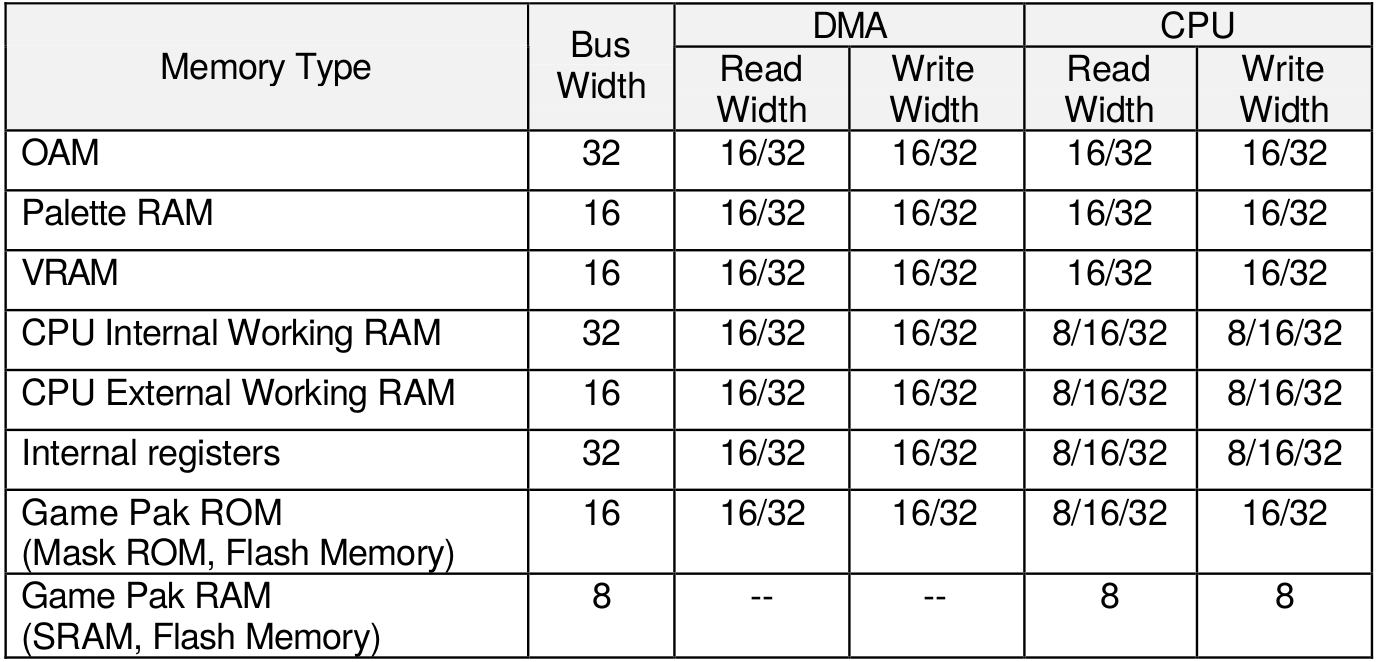
\includegraphics[width=14cm, keepaspectratio=true]{accesstimes}
	\end{figure}\cite{GBAManual}
\end{center}
	\subsection{Memory Interface}
	The memory interface is a bus, shared by the DMA controller and the CPU. Bus contention is avoided by priority - if a DMA is ready, the CPU is paused until the DMA completes. Neither the CPU nor the DMA can write to VRAM, OAM, or Palette RAM until either \texttt{VBLANK} or \texttt{HBLANK} regions of the VGA cycle. Outside of \texttt{VBLANK} or \texttt{HBLANK}, the graphics pipeline assumes exclusive ownership of VRAM, OAM, and Palette RAM, and the CPU/DMA bus is electrically disconnected (High-Impedence) from the graphics memory. During \texttt{VBLANK} and \texttt{HBLANK}, the CPU/DMA bus drives the bus for graphics memory as well.\\\\
	Bus accesses are sent to the memory controller, where they are forwarded to the memory region in which the address lies. If a system attempts to make an access to an undefined region, either the system will enter an error state, or the bus \texttt{ABORT} signal will be set high, depending on whether our target games make accesses to undefined regions during standard operation. If the latter is the case, we also have the option of mirroring undefined addresses onto defined regions (a step that the GBA does internally, but that isn't documented in the programmer's guide). The system is little endian.\\
	
	\subsection{Memory Timings}
	Each region of the memory also has a specific access time. Specifically, this is where the three Game Pak ROM regions differ, in the case of the first region, WS0 denotes that zero wait states should be used in the access, for the second, WS1 denotes that one wait state should be used in the access, and so on. The length of a wait state depends on the state of the \texttt{WAITCNT} MMIO register. In the GBA system, accesses also recieve a speedup when they are sequential. We do not plan to implement this, since DRAM and BRAM both give single cycle access. If it turns out that the timing differences are necessary for standard operation, we can implement delays for random accesses by asserting the \texttt{WAIT} bus signal as necessary. Different regions of GBA memory also have different access times associated with them - our plan of action is the same for this.\\\\
	
	Read and Write timings for our system are detailed below. \texttt{WRITE} is the write enable signal, \texttt{RDATA} is data from a memory read, \texttt{WDATA} is data for a memory write, and \texttt{ADDR} is the address for the access to occur at. Vertical lines indicate positive edges of the clock.
	\begin{verbatim}
	Read Access:
	ADDR   |<Address1>|<Address2>|------------|
	RDATA  |----------|--<Data1>-|--<Data2>---|
	
	Write Access:
	ADDR   |<Address1>|<Address2>|-----------|
	WDATA  |----------|--<Data1>-|--<Data2>--|
	WRITE  |--<High>--|--<High>--|--<Low>----|
	\end{verbatim}
	
	\subsection{Memory Region Access Timings}
	\begin{verbatim}
	    Region        Bus   Read      Write     Cycles
	    BIOS ROM      32    8/16/32   -         1/1/1
	    Work RAM 32K  32    8/16/32   8/16/32   1/1/1
	    I/O           32    8/16/32   8/16/32   1/1/1
	    OAM           32    8/16/32   16/32     1/1/1 *
	    Work RAM 256K 16    8/16/32   8/16/32   3/3/6 **
	    Palette RAM   16    8/16/32   16/32     1/1/2 *
	    VRAM          16    8/16/32   16/32     1/1/2 *
	    GamePak ROM   16    8/16/32   -         5/5/8 **/***
	    GamePak Flash 16    8/16/32   16/32     5/5/8 **/***
	    GamePak SRAM  8     8         8         5     **
	    Timing Notes:
	    *   Plus 1 cycle if GBA accesses video memory at the same time.
	    **  Default waitstate settings, see System Control chapter.
	    *** Separate timings for sequential, and non-sequential accesses.
	    One cycle equals approx. 59.59ns (ie. 16.78MHz clock).
	    Sequential vs Random access timings on p.23 of Nintendo GBA doc
	    All memory (except GamePak SRAM) can be accessed by 16bit and 32bit DMA.
	    \end{verbatim} \cite{GBATek}
	
	\section{CPU}
	The GBA uses an ARM7TDMI processor, implementing the ARMv4t ISA, which operates on a three-stage pipeline (fetch, decode, execute). When an instruction in the execute stage will take more than one cycle to complete, the CPU stalls the pipeline until the instruction completes. For branches, the CPU flushes the fetch and decode stages, reloading from the address that was branched to. The CPU also (per ARM specification) can switch between 32-bit ARM instruction mode and 16-bit THUMB instruction mode via the \texttt{BX} instruction. During execution, the program has accesses to 17 registers, with R13, R14, and SPSR swtiched between several banks depending on execution mode.\\\\
	We had planned to get most of the CPU from an outside source, then implement the necessary features. Our options were either the Storm Core from OpenCores, the ARM9 chip embedded on the Zedboard, or a version of the ARM7TDMI that some engineer wrote between jobs. Interestingly, the core from some random engineer seemed the most promising since THUMB mode was partially implemented already. The Storm Core had no infrastructure for THUMB mode in place, as well as some other issues, and the ARM9 core had some backwards compatibility issues between ISA versions that we wouldn't be able to implement hardware fixes for.
	
	\subsection{CPU Interface}
	The ARM7TDMI core that we got didn't have all the signals that are described in the ARM7TDMI specification. In fact, most of the signals were missing. The ARM7TDMI was a fairly popular processor, designed for a much more general purpose than the GBA, so many of the signals were unnecessary for our context. Namely, the JTAG debug interface (the D in TDMI), and the EmbeddedICE macrocell (the I in TDMI) were intended for post-silicon verification - a process that is wholly unnecessary for our project. The processor also allows for a choice between unidirectional and bidirectional data buses, which we also don't need - we picked unidirectional and stuck with it. We also don't use the coprocessor interface - it was used in the GBA to provide backwards compatibility with Game Boy Color games (interfacing with a Z80 processor). All in all, the signals that we actually need for our interface is an aggressive subset of the signals specified in the ARM7TDMI documentation - if the core we got online didn't have it and we could justify not including it, we didn't. We lose cycle accuracy, but that was never a primary goal of the project and it seems easier to adhere to approximate cycle timings in the context of our system than try to replicate cycle timings that we don't have access to. Again, the primary issue due to our lack of cycle accuracy is memory accesses occurring faster than they should, but we can add wait timings to try to replicate the original timings (or to get closer to them).\\\\\
	The interface from the CPU to the rest of the system is as follows:
	\begin{verbatim}
	input  logic CLK,          // The system clock
	input  logic PAUSE,        // Pause the CPU when high (for wait states)
	input  logic DMAActive     // Pauses CPU and sets memory output bus signals to 'Z
	input  logic nRESET,       // System reset
	
	-- Interrupts
	input  logic nIRQ          // Interrupt Request
	
	-- Memory interface
	output logic [31:0] ADDR,  // Memory Address
	output logic [31:0] WDATA, // Write Data
	input  logic [31:0] RDATA, // Read Data
	input  logic ABORT,        // ABORT memory access
	output logic WRITE,        // Write enable
	output logic [1:0] SIZE,   // Memory write size
	\end{verbatim}
	The module header for the core also includes a \texttt{FIQ} signal for fast interrupts, but the GBA doesn't use these. The signal's integrated in the logic for the core - it seemed like an unnecessary amount of work to remove it. 
	
	\subsection{Interrupts}
	The CPU has a single interrupt request line, but can receive interrupts from 14 different sources. This is managed via the Interrupt Controller, along with a couple MMIO registers. The CPU's nIRQ line is set to the OR of all incoming interrupts that have not been masked (masking in Interrupt Master Enable and Interrupt enable registers). When an interrupt is received, the CPU enters nIRQ mode, then examines the Interrupt Request (IF) MMIO register to determine the source of the interrupt. Interrupt priority is handled by software \cite{GBAManual}.\\\\
	An interrupt can be generated by the following sources:
	\begin{multicols}{3}
	\begin{itemize}
		\item GamePak (IF[13]) % TODO Info!!
		\item Key Press (IF[12])
		\item DMA{0-3} Transfer (IF[11-8])
		\item Link Cable Communication (IF[7])
		\item Timer Overflow (IF[6-3])
		\item V Count match (IF[2])
		\item HBLANK (IF[1])
		\item VBLANK (IF[0])
	\end{itemize} 
	\end{multicols}
	
	\section{DMA}
	The GBA has 4 DMA channels numbered 0 to 3. Only one DMA channel can be operating at once, so DMA channel 0 has the highest priority, 1 has the second, and so on. When a higher priority channel preempts a lower priority channel, the lower priority channel is paused until the higher priority channel completes. As stated earlier, all DMA channels have priority over the CPU with respect to the memory bus.\\\\
	Individual DMA channels differ slightly in expected use. DMA0, naturally, is used for high priority transfers (feeding graphics during HBLANK) and cannot be used to transfer from GamePak ROM, DMA1 and DMA2 can be used to feed DMA sound channels, and DMA3 can be used to transfer data from GamePak ROM.\\\\
	For each DMA, the source address is specified in MMIO \texttt{REG\_DMA*SAD}, the destination address in \texttt{REG\_DMA*DAD}, the number of words or half-words to transfer in \texttt{REG\_DMA*CNT\_L[13:0]}.
	General controls are set in \texttt{REG\_DMA*CNT\_H[15:0]}, including whether the count is the number of words or half-words, whether the transfer will repeat, when the DMA will start, enables, and whether the DMA will generate a CPU interrupt upon transfer completion ~\cite{GBAManual}.
	
	\section{Graphics}
	The Game Boy Advance graphics pipeline uses a combination of backgrounds and sprites, which the GBA refers to as objects. There are three types of backgrounds - Character backgrounds, where the screen is composed of tiles that specify colors in a palette, Rotation/Scaling backgrounds, where the screen is tiled, but the tiles can be scaled or rotated (but fewer can be used), and Bitmap backgrounds, where the entire screen is specified pixel-by-pixel with colors specified in a palette. All backgrounds can be flipped vertically or horizontally. The background mode (specified in DISPCNT) controls how many backgrounds, and which types of backgrounds, can be used. \cite{GBAManual}
	
	\subsection{Objects}
	Objects are stored in character mode, where pixels index into a palette for color values. Limits on objects, like the number of objects that can display and which palettes are used, are determined by the background mode. Parameters for objects are specified in OAM in sets of 4 bytes, or 2 bytes when using bitmapped backkgrounds (Background mode 3-5). Objects are given a priority (from 0-3) as part of the parameters, with 0 taking the highest priority. \cite{GBAManual}
	
	\subsection{Priority}
	Objects with priority 0 have the highest priority. Backgrounds with priority zero are next, then objects with priority 1, then backgrounds with priority 1, and so on. The backdrop has the lowest priority, which is just a default color if the color for a given pixel are unspecified. If objects or backgrounds are transparent, the transparent color (color 0) is used (specified in the palette). \cite{GBAManual}. 
	
	\subsection{Windowing}
	The Game Boy Advance has a notion of windows, where objects and backgrounds inside the windows can be collectively turned on or off. The size and location of the windows are set in MMIO registers. Window 0 has a higher display priority than window 1. \texttt{REG\_WININ} is used to control whether BG3, BG2, BG1, BG0, or objects are turned on or off. \cite{GBAManual}
	
	\subsection{Mosaics}
	Backgrounds and sprites can be drawn with a mosaic, where some number of dots of a normal display should comprise a large dot. Specifically, starting from the top-left corner, a block of size \{H size * V Size\} will be the same color as the top-left corner. This has the effect of dividing the screen into \{H size * V Size\} chunks, where blocks on the edges will be smaller if the background/object can't be evenly divided into chunks. All background are set to the same mosaic size (if one is specified), the same holds for all sprites. Mosaic information is specified in \texttt{REG\_MOSAIC}.\cite{GBAManual}
	
	\subsection{VGA Display}
	Natively, the GBA expects a 240x160 resolution - a 3:2 aspect ratio. This doesn't exist in modern monitors. Originally, we had planned to output 480x640 VGA, but the GBA documentation didn't give us pulse width timings. In the end, we decided to double buffer the display, storing the double buffer in the Zedboard's BRAM. The graphics pipeline writes the color data that will be output to the double buffer controller and asserts that the buffers should switch at the end of a display cycle (\texttt{toggle}). The VGA controller presents the buffer address for the next pixel (since reads are sequential from BRAM) and writes the data read from the buffer to \texttt{VGA\_R[3:0], VGA\_B[3:0], VGA\_G[3:0]}. The VGA is clocked at three times the system clock (16.78Mhz), so that both the VGA controller and the graphics pipeline stay coordinated on a per-frame basis. 
	
	\section{Audio}
	The GBA has four wave sound channels and two DMA sound channels. The wave channels are identical to the Game Boy Color, with each channel having slightly capabilities. Channel 1 generates a square wave tone with optional frequency sweep, channel 2 generates a rectangular tone, channel 3 generates a sawtooth wave, and channel 4 generates white noise. Both DMA channels operate the same way - each specifies a timer that will be used to trigger transfers from the FIFO to the audio circuit, and each is given an 8 word FIFO for sound data. DMA requests are triggered to refill the FIFOs when a transfer causes the FIFO to have fewer than 4 words. ~\cite{GBAManual}.
	
	\subsection{Zedboard Audio Codec}
	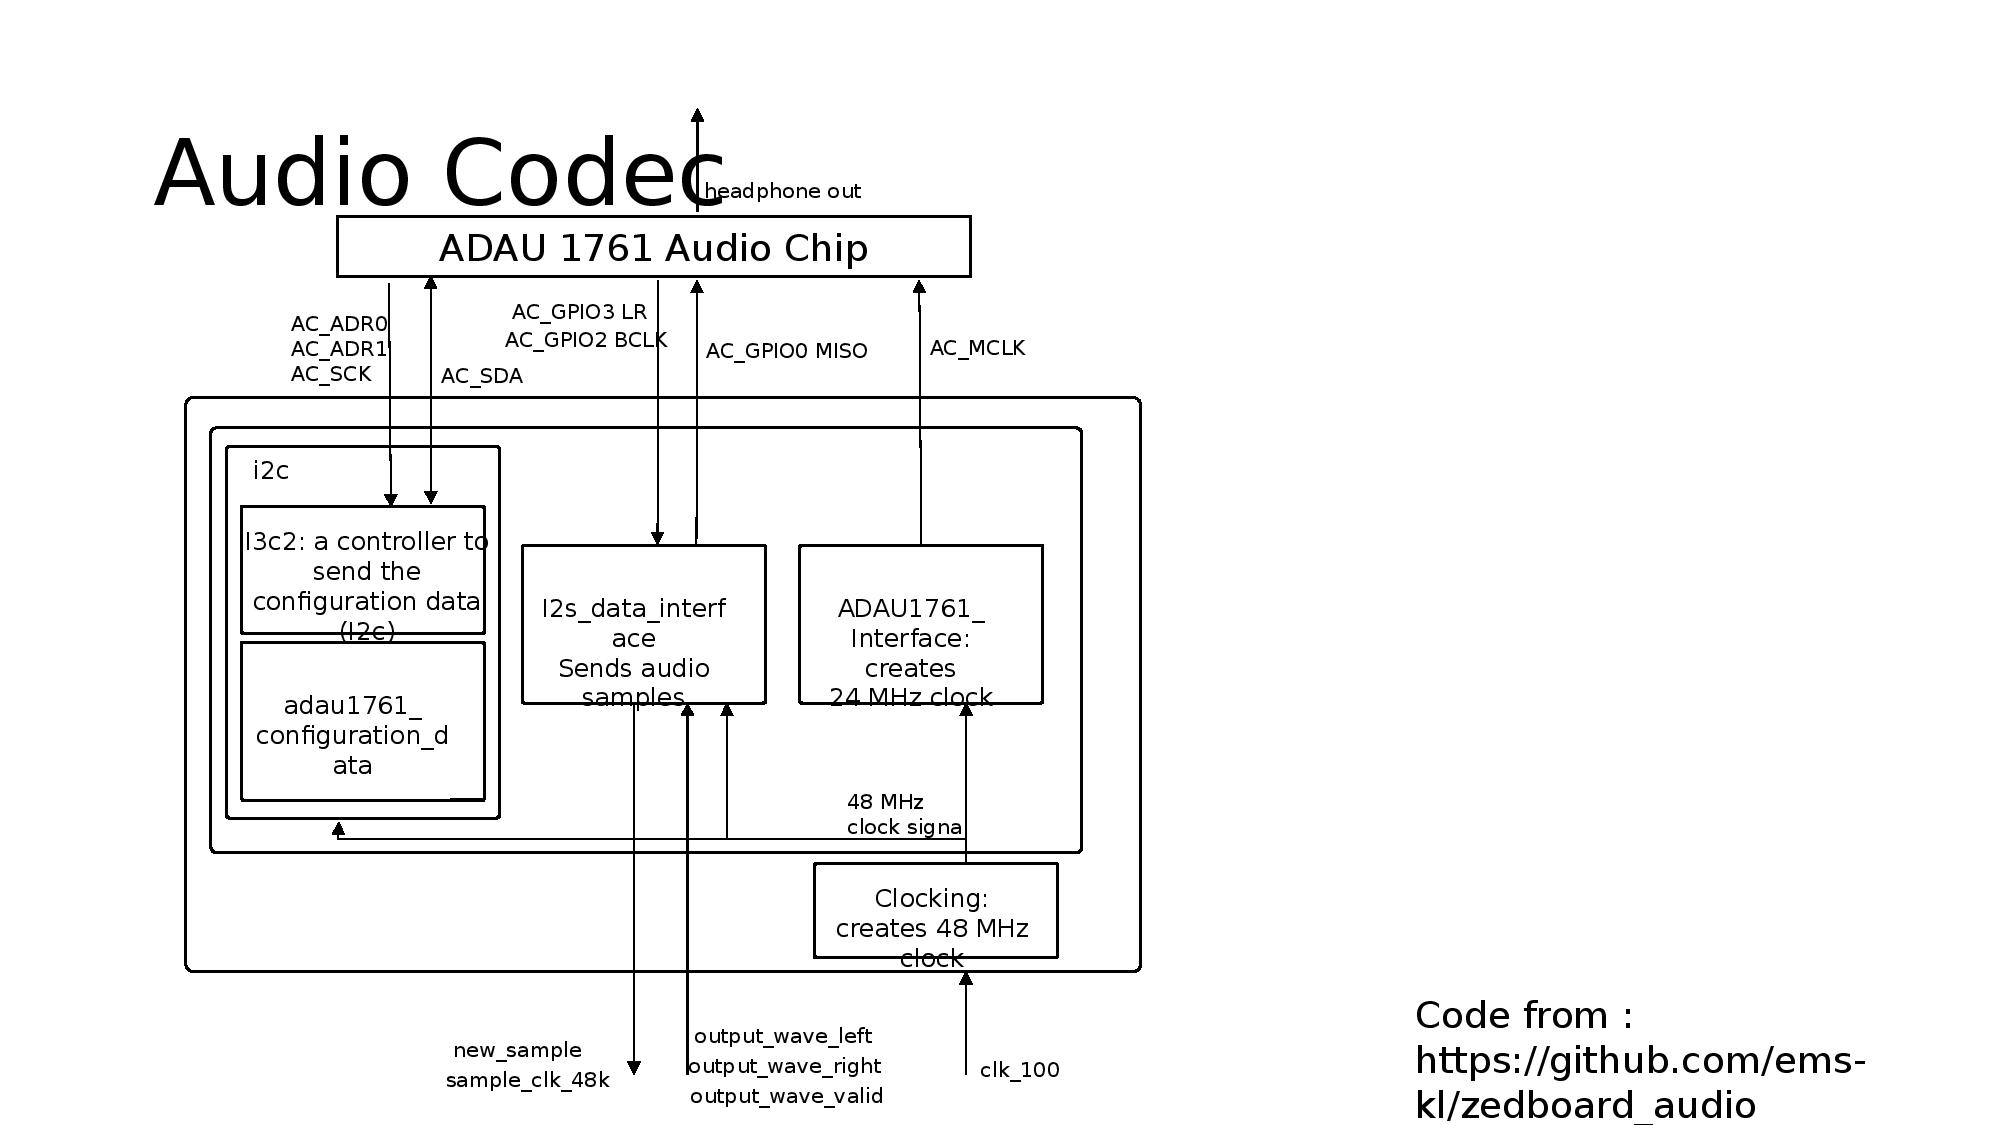
\includegraphics[width=14cm, height=15cm, keepaspectratio=true]{codec}
	
	\section{Timers}
	The Game Boy Advance, per specification, has 4 16-bit timers that are programmed via registers TM{0-3}CNT\_{L,H}. These timers can be programmed to count at the system clock rate, or at 1/64th, 1/256th, or 1/1024th of the system clock rate. Each timer can also generate an interrupt when the timer count overflows the 16 bit TM{0-3}CNT\_L register.\\
	
	\section{Controller}
	We use an SNES controller connected to one of the Zedboard's PMOD ports. The controller is connected as follows:
	\begin{verbatim}
	       ----------------------------- ---------------------
	       |                             |                      \
	       | (1)     (2)     (3)     (4) |   (5)     (6)     (7) |
	       |                             |                      /
	       ----------------------------- ---------------------
	       
	       Pin     Description             Zedboard Connection
	       ===     ===========             ======================
	       1       +5v                     Zedboard +5V
	       2       Data clock              JA3
	       3       Data latch              JA2
	       4       Serial data             JA1
	       5       ? (+5v)                 no wire
	       6       ? (+5v)                 no wire
	       7       Ground                  JA GND
	\end{verbatim}
	As detailed above, the Zedboard expects a +5V VDD, whereas the PMOD connectors output at +3.3V. To avoid frying the Zedboard, we used a \textit{Sparkfun Level Converter}.\\\\
	The serial protocol between the controller module on the Zedboard and the SNES controller begins with the CPU sending a 12us wide positive pulse on the Data Latch pin. The CPU wait 6us, then sends 16 data clock pulses, beginning with the negative edge of the clock, that are 50\% duty cycle with a 12us period on Data Clock (Data Clock is high when idle). The Controller shifts latched button states on the positive edge of the Data Clock, and the CPU samples the Serial Data line for button state on the negative edge. Button state is reported active-low. In our implementation, button state is reported in the order below:\\
	\begin{verbatim}
	Clock Cycle     Button Reported
	===========     ===============
	0               Y
	1               Select
	2               Start
	3               Up on joypad
	4               Down on joypad
	5               Left on joypad
	6               Right on joypad
	7               A
	8               X
	9               L
	10              R
	11              none (always high)
	12              none (always high)
	13              none (always high)
	14              none (always high)
	15              B
	\end{verbatim}
	This is not strictly according to the SNES controller specification, but it is consistent. The serial protocol repeats at 60Hz.
	
	\section{Results}
	
	\subsection{Status}
	
	\section{Vivado Tips and Tricks}
	
	\section{Lessons Learned}
	
	\section{For groups that want to finish this project}

	
	
	\section{Plan of Attack}
	\subsection{Current State}
	Currently, the DMA is code complete and untested, the graphics pipeline has been completely design, 4 channel sound is working according to specification, the controller interface is complete and verified, and the CPU runs 100000+ cycles of BIOS code without entering undefined state, although it does infinite loop. The CPU is, however, in a state where system integration can begin with custom roms - we have infrastructure in place to create these from C code. \\\\
	The sound system had some roadblock - it's pretty difficult and annoying to debug sound. With 4 channel working, DMA should come reasonably quickly. The lack of concrete THUMB support in the CPU put the system a couple weeks behind, but bugs are being fixed on a daily basis and there seem to be relatively few left (but, granted, it's impossible to tell). 
	
	\subsection{Next Steps}
	We plan to have DMA sound working on a system level within a week. In this, the CPU ROM will be preloaded with a custom ROM to initialize the DMA and sound channel, sound data will be preloaded in some memory (hopefully DRAM), then playback will start. 
	
	\printbibliography
	
\end{document}